\documentclass[10pt,xcolor={dvipsnames},aspectratio=169]{beamer}
%\documentclass[10pt,xcolor={dvipsnames},aspectratio=169,trans,compress]{beamer}
%\documentclass[10pt,xcolor={dvipsnames},handout]{beamer}

% option passed to the theme
\usetheme[
  font={default}, % serif, sans, helvet, times, kp (sans is default)
  color={default} % forest, navy, dark, IEEE, UHRed, UHCullen (UHCullen is default)
%  language={american}, % american, british, spanish, ... (american is default)
%  progressstyle={none},   % default, noNumber, none
%  sidebarnone, % sidebarleft, sidebarright (sidebarright is default)
%  showallsubsections, % hideothersubsections, hideallsubsections (hideothersubsections is default)
]{UHCullen}

%-------------------------------------------------------
% Configure citations
%-------------------------------------------------------

% add two files
\addbibresource{bib/ref_nn.bib}
\addbibresource{bib/ref_superrs.bib}

%-------------------------------------------------------
% INDIVIDUAL COLORS
%-------------------------------------------------------

% The elements of the template can be changed individually. Note that you may
% need to use different colors in beamer / handout mode, when using the following
% methods:

% Change the bar colors:
% \setbeamercolor{UHCullen}{fg=NavyBlue!10,bg=NavyBlue}
% \setbeamercolor{UHBackground}{fg=NavyBlue!8,bg=white}

% Change the color of the structural elements:
% \setbeamercolor{structure}{fg=NavyBlue}

% Change the frame title text color:
% \setbeamercolor{frametitle}{fg=black!5,bg=NavyBlue}

% Change the normal text colors:
% \setbeamercolor{normal text}{fg=black!75,bg=gray!5}

% Change the block title colors
% \setbeamercolor{block title}{use=UHCullen, bg=UHCullen.bg!20!black, fg=UHCullen.fg} 

%-------------------------------------------------------
% IMAGE FILES
%-------------------------------------------------------

% optional, set the logo on the title page.
% \setTitleLogo{UHCullenGraphics/logo-cullen-color}

% optional, set the logo on each frame.
% \setLogo{UHCullenGraphics/logo-cullen-color}

% optional, set the logo on the final page.
% \setFinalLogo{UHCullenGraphics/logo-cullen-long}

% optional, the following options only works in classic / colored mode.
% set the height of the title figures.
% \setlength{\titlefigureheight}{0.2\paperheight}

% optional, the following options only works in classic mode.
% use only one figure on the title page.
% \setTitleImageA[width=\paperwidth]{UHCullenGraphics/cullen-1}
% \setTitleImageB{}
% \setTitleImageC{}

% use two figures on the title page.
% \setTitleImageA[width=0.5\paperwidth]{UHCullenGraphics/cullen-1}
% \setTitleImageB[width=0.5\paperwidth]{UHCullenGraphics/cullen-2}
% \setTitleImageC{}

% use three figures on the title page.
% \setTitleImageA{UHCullenGraphics/cullen-1}
% \setTitleImageB{UHCullenGraphics/cullen-2}
% \setTitleImageC{UHCullenGraphics/cullen-3}

% optional, set the background image to the final page, only works in classic mode.
% \setFinalImage[height=\paperheight-0.9cm]{UHCullenGraphics/cullen-final}

%-------------------------------------------------------
% INCLUDE PACKAGES
%-------------------------------------------------------

\usepackage{metalogo}

%-------------------------------------------------------
% INFORMATION IN THE TITLE PAGE
%-------------------------------------------------------

% [] is optional - is placed on the bottom of the sidebar on every slide
\title[UHCullen Theme]
{ % is placed on the title page
  \textbf{The UHCullen Beamer Theme}
}

% subtitle is optional.
\subtitle[v. 1.2.1]
{
\textbf{v. 1.2.1}
}

% author is required. Use \texorpdfstring to configure hyperref correctly.
\author[Author 1]
{Author 1\texorpdfstring{\footnotemark[1]}{},
Author 2\texorpdfstring{\footnotemark[2]}{},
\texorpdfstring{$\cdots$}{...}
\texorpdfstring{ \\
  {\ttfamily author1@gmail.com}
}{}}

% institute is required. Will be shown in the title.
\institute[]
{%
  \footnotemark[1]Affiliation 1\\
  \footnotemark[2]Affiliation 2
}

% date is required. will be shown on each page.
\date{\today} % Could be configured as \today or a manually specified date: \formatdate{day}{month}{year}

%-------------------------------------------------------
% THE BODY OF THE PRESENTATION
%-------------------------------------------------------

\begin{document}

%-------------------------------------------------------
% THE TITLEPAGE
%-------------------------------------------------------

\titleframe

\begin{frame}{Content}{}
\tableofcontents
\end{frame}

%-------------------------------------------------------
\section{Introduction}
%-------------------------------------------------------
\subsection{License}
\begin{frame}{Introduction}{License}
%-------------------------------------------------------

  \begin{itemize}
    \item<1-> This template is inspired by \chref{https://www.overleaf.com/latex/templates/beamer-presentation-template-feather-theme/jcbpcdxqbxbf}{Feather theme}. Some of the implementations are copied from \chref{http://tug.ctan.org/macros/latex/contrib/beamer/base/themes/outer/beamerouterthemesidebar.sty}{sidebar outer theme} and \chref{http://tug.ctan.org/macros/latex/contrib/beamer/base/themes/outer/beamerouterthememiniframes.sty}{miniframes outer theme}. The GPLv3 is copied from the original templates to this one.
    \item<2-> The \texttt{beamer} (default) style of this template is modified according to the standard of \chref{https://www.egr.uh.edu/office-communications/resources}{UH Cullen PPT templates}. Three different styles are implemented as \texttt{beamer} mode, \texttt{trans} mode, and \texttt{handout} mode.
    \item<3-> The rest of the theme is provided under the GNU General Public License v. 3 (GPLv3) \chref{http://www.gnu.org/licenses/}{http://www.gnu.org/licenses/}. This means that you can redistribute it and/or modify it under the same license. 
  \end{itemize}
\end{frame}

%-------------------------------------------------------
\section{Installation}
%-------------------------------------------------------
\subsection{Source files}
\begin{frame}{Installation}{Source files}
%-------------------------------------------------------

\onslide<1->{
  \begin{block}{}
  The basic theme contains 2 source files, they are shared by all modes:
    \begin{itemize}
      \item {\tt beamerthemeUHCullen.sty}
      \item {\tt beamercolorthemeUHCullen.sty}
    \end{itemize}
  \end{block}
}

\only<1|trans:1|handout:1>{
  \begin{block}{}
    The default \texttt{beamer} mode is provided by the following sub-themes. The template is designed based on the \chref{https://www.egr.uh.edu/sites/ccoe.egr.uh.edu/files/files/standard_uh_cce_powerpoint_presenation_for_faculty_and_staff.pptx}{Classic PPT template}. These files can be used individually.
    \begin{itemize}
      \item {\tt beamerouterthemeUHCullenClassic.sty}
      \item {\tt beamerinnerthemeUHCullenClassic.sty}
    \end{itemize}
  \end{block}
}

\only<2|trans:2|handout:2>{
  \begin{block}{}
    The transparency (\texttt{trans}) mode is provided by the following sub-themes. Some styles are simplified in this mode. The template is designed based on the \chref{https://www.egr.uh.edu/sites/ccoe.egr.uh.edu/files/files/option2presentationslide.pptx}{Red-on-white PPT template}. These files can be used individually.
    \begin{itemize}
      \item {\tt beamerouterthemeUHCullenColored.sty}
      \item {\tt beamerinnerthemeUHCullenColored.sty}
    \end{itemize}
  \end{block}
}

\only<3|trans:3|handout:3>{
  \begin{block}{}
    The \texttt{handout} mode is provided by the following sub-themes. This model provide minimal features and the simplest style. The template is designed based on the \chref{https://www.egr.uh.edu/sites/ccoe.egr.uh.edu/files/files/option1presentationslide.pptx}{Standard PPT template}. These files can be used individually.
    \begin{itemize}
      \item {\tt beamerouterthemeUHCullenColored.sty}
      \item {\tt beamerinnerthemeUHCullenColored.sty}
    \end{itemize}
  \end{block}
}

\end{frame}

%-------------------------------------------------------
\subsection{Local and Global installation}
\begin{frame}{Installation}{Local and Global installation}
%-------------------------------------------------------
  The theme can be installed for \textbf{local} or \textbf{global} use.
  \begin{block}{Local Installation}
    \small \begin{itemize}    
      \item Local installation is the simplest way of installing the theme. 
      \item You need to placing the 8 source files in the same folder as your presentation. When you download the theme, the 8 theme files are located in the {\tt local} folder.
    \end{itemize}
  \end{block}
  \begin{block}{Global Installation}
    \small \begin{itemize}
      \item If you wish to make the theme globally available, you must put the files in your local latex directory tree. The location of the root of the local directory tree depends on your operating system and the latex distribution. 
      \item Detailed steps on how to proceed installation under various operating systems can be found at Beamer documentation.
    \end{itemize}
  \end{block}
\end{frame}
     

%-------------------------------------------------------
\subsection{Required Packages}
\begin{frame}{Installation}{Required Packages}
%-------------------------------------------------------

  For using the basic \texttt{UHCullen} Theme you will need the Bemaer class installed and the following 5 packages
  \begin{itemize}
    \item \texttt{TikZ}\footnote{TikZ is a package for creating beautiful graphics. Have a look at these \chref{http://www.texample.net/tikz/examples/}{online examples} or the \chref{http://tug.ctan.org/tex-archive/graphics/pgf/base/doc/generic/pgf/pgfmanual.pdf}{pgf user manual}.}
    \item \texttt{tcolorbox}\footnote{tcolorbox is a package for creating customized blocks. To learn details, see \chref{http://tug.ctan.org/tex-archive/macros/latex/contrib/tcolorbox/tcolorbox.pdf}{tcolorbox user manual}.}
    \item \texttt{datetime}\footnote{datetime is required for formatting the date.}
    \item \texttt{textcase}\footnote{textcase is required for providing uppercase filter.}
    \item \texttt{calc}\footnote{calc is required for calculating the space and length of the object in this templates.}
  \end{itemize}
  These packages are required to be included in your~\LaTeX~distribution.
\end{frame}

\begin{frame}{Installation}{Required Packages}
More required packages for advanced utilities:
\begin{itemize}
  \item \textbf{Citation}: \texttt{csquotes}, \texttt{biblatex}\footnote{biblatex is the best way to show citations in beamer, however, it may cause compatibility problems.}, \texttt{cleveref}\footnote{cleveref is the best way to create auto references, however, it may cause compatibility problems.}
  \item \textbf{Font}: \texttt{fontenc}
  \item \textbf{Environment}: \texttt{float}, \texttt{algorithm}, \texttt{algorithmic}, \texttt{subfigure}
  \item \textbf{Conditions}: \texttt{ifthen}, \texttt{ifxetex}
  \item \textbf{Others}: \texttt{tabularx}, \texttt{array}, \texttt{siunitx}, \texttt{colortbl}
\end{itemize}
\end{frame}

%-------------------------------------------------------
\section{User Interface}
\subsection{Loading Beamer}
\begin{frame}{User Interface}{Loading Beamer with different mode}
%-------------------------------------------------------
  \vspace{-0.5em}
  \begin{block}{The Beamer Mode}
    \small
    The UHCullen can be loaded in two different \texttt{beamer} modes. The default mode is\\
    {\tt \textbackslash documentclass[<options>]\{beamer\}}\\
    Here \texttt{<options>} can be \texttt{beamer} (by default), \texttt{trans}, or \texttt{handout}.
  \end{block}
  \begin{block}{The Page Size}
    \small
    The size of the page can be configured in class options\\
    {\tt \textbackslash documentclass[aspectratio=169]\{beamer\}}\\
    {\tt \textbackslash documentclass[aspectratio=43]\{beamer\}}\\
    According to the standard of UHCullen, we recommend users to use 16:9 in \texttt{beamer} (presentation) mode.
  \end{block}
\end{frame}


%-------------------------------------------------------
\subsection{Loading the Theme and Theme Options}
\begin{frame}{User Interface}{Loading the Theme and Theme Options}
%-------------------------------------------------------
  \vspace{-0.5em}
  \begin{block}{The Presentation Theme}
    \small
    The UHCullen Theme can be loaded in a familiar way. In the reamble of your {\tt tex} file you must type\\
    {\tt \textbackslash usetheme[<options>]\{UHCullen\}}\\
    The presentation theme loads the inner, outer and color UHCullen theme files and passes the {\tt <options>} on to these files.
  \end{block}
  \begin{block}{The Inner and Outher Themes}
    \small
    Take the Classic Theme as an example. If you wish you can load only the inner, or the outher theme directly by\\
    {\tt \textbackslash useinnertheme\{UHCullenClassic\}} (and it has no options)\\
    {\tt \textbackslash useoutertheme[<options>]\{UHCullenClassic\}} (it has several options)\\
    \begin{itemize}
      \item details about the available options can be referred in the ReadMe file.
    \end{itemize}
  \end{block}
\end{frame}

\begin{frame}{User Interface}{Loading the Theme and Theme Options}
  \begin{block}{The Color Theme}
    \small
    Also you can load only the color theme by writing in the preamble of the {\tt tex} file 
    \begin{itemize}
      \item {\tt \textbackslash usecolortheme[font=<fontname>,color=<palette>]\{UHCullen\}}
    \end{itemize}
    The fonts and colors can be configured by options.

    We can also change the colors of the various elements by
    \begin{itemize}
      \item Change the bar colors: \\    
      {\tt \textbackslash setbeamercolor\{UHCullen\}\{fg=<color>, bg=<color>\}}
  
      \item Change the background colors: \\    
      {\tt \textbackslash setbeamercolor\{UHBackground\}\{fg=<color>, bg=<color>\}}
  
      \item Change the color of the structural elements: \\    
      {\tt \textbackslash setbeamercolor\{structure\}\{fg=<color>\}}
    \end{itemize}
  \end{block}
\end{frame}


%-------------------------------------------------------
\subsection{TeX Compiler}
\begin{frame}{User Interface}{TeX Compiler}
  %-------------------------------------------------------
  \begin{block}{Preferred Compiler}
    The preferred compiler of this template is pdf\LaTeX. All features work properly with this compiler.
  \end{block}
  \begin{block}{Compatible mode}
    This template is also compatible with \XeLaTeX. However, the following features may fall back to the compatible mode.
    \begin{itemize}
      \item The background of \texttt{Classic outer theme} may look slightly different due to the bug of \texttt{\textbackslash tikzfading}.
      \item Some fonts like \texttt{helvetical} may fall back to alternatives.
    \end{itemize}
  \end{block}
\end{frame}


%-------------------------------------------------------
\subsection{Customize images}
\begin{frame}{User Interface}{Customize Images}
%-------------------------------------------------------
\only<1|trans:1|handout:1>{
\begin{block}{The Title and Final Logo}
  \small 
  \begin{itemize}
    \item Use the following command to change the logo on the title page (the recommended w:h ratio is \texttt{5:2}.):\\
    {\tt \textbackslash setTitleLogo\{<path-to-the-logo>\}}
    \item Use the following command to change the logo on the final page (the recommended w:h ratio is \texttt{14:1}.):\\
    {\tt \textbackslash setFinalLogo\{<path-to-the-logo>\}}
  \end{itemize} 
\end{block}
}
\only<2|trans:2|handout:2>{
\begin{block}{The Frame Logo}
  \small 
  \begin{itemize}
    \item Use the following command to change the logo on each frame:\\
    {\tt \textbackslash setLogo\{<path-to-the-logo>\}}
    \item An optional argument could be specified for providing a different w:h ratio.):\\
    {\tt \textbackslash setLogo[<ratio>]\{<path-to-the-logo>\}}
  \end{itemize} 
\end{block}
}
\end{frame}

\begin{frame}{User Interface}{Customize Images}
\only<1|trans:1|handout:1>{
\begin{block}{The Title Images}
  \small 
  There are three images (ImageA, ImageB, and ImageC) that can be changed on the title page of the Classic theme:
  \begin{itemize}
    \item For each image (like ImageA), a file path can be provided by:\\
    {\tt \textbackslash setTitleImageA\{<path-to-the-file>\}}
    \item More \texttt{\textbackslash includegraphics} options can be given by the optional argument:\\
    {\tt \textbackslash setTitleImageA[<options>]\{<path-to-the-file>\}}
  \end{itemize} 
\end{block}
}
\only<2|trans:2|handout:2>{
\begin{block}{The Final Images}
  \small 
  Only one image can be changed on the final page of the Classic theme:
  \begin{itemize}
    \item The image file path can be provided by:\\
    {\tt \textbackslash setFinalImage\{<path-to-the-file>\}}
    \item More \texttt{\textbackslash includegraphics} options can be given by the optional argument:\\
    {\tt \textbackslash setFinalImage[<options>]\{<path-to-the-file>\}}
  \end{itemize} 
\end{block}
}
\end{frame}


%-------------------------------------------------------
\section{Examples}
\begin{frame}{Examples}{Citations}
%-------------------------------------------------------
\begin{itemize}
  \item This is the template for UH slides, which includes:
  \begin{itemize}
    \item \textbf{Table}: Check \cref{tab:params}.
    \item \textbf{Figure}: Check \cref{fig:ex1:resD}.
    \item \textbf{Block and Equation}: Check \eqref{fml:eq1:partialW}.
    \item \textbf{Theorem}: Check \cref{thm:th1}.
    \item \textbf{Algorithm}: Check \cref{alg::Algorithm}.
  \end{itemize}
\end{itemize}
\begin{block}{Citation block}
  And here we would like to test the references: \textit{Zeiler et al.}\footcite{Zeiler5539957}, \textit{Yang et al.}~\footcite{Yang6175956}, \textit{Dong et al.}~\footcite{Dong7115171}.
\end{block}
\end{frame}


%-------------------------------------------------------
\begin{frame}{Examples}{Table}
%-------------------------------------------------------
\begin{itemize}
  \item Test table, which is shown in \cref{tab:params}.
\end{itemize}

\begin{table}[htbp]
  \centering
  \normalsize
  \caption[Parameters of Daubechies's filter.]{Parameters of \textit{Daubechies}'s filter.}
  \label{tab:params}
  \begin{tabular}{|c|c|c|}
    \hline
    $n$ & $h[n]$ & $g[n]$ \\ \hline
    0 &  0.3327 & -0.0352 \\ \hline
    1 &  0.8069 & -0.0854 \\ \hline
    2 &  0.4599 &  0.1350 \\ \hline
    3 & -0.1350 &  0.4599 \\ \hline
    4 & -0.0854 & -0.8069 \\ \hline
    5 &  0.0352 &  0.3327 \\ \hline
  \end{tabular}
\end{table}
\end{frame}


%-------------------------------------------------------
\begin{frame}{Examples}{Figures}
%-------------------------------------------------------
\begin{itemize}
  \item Test inner subgraphs, i.e. \cref{fig:ex1:resD:a} and \cref{fig:ex1:resD:b}.
\end{itemize}

\begin{figure}[htbp]
  \centering
  \subfigure[$D=1$]{ \label{fig:ex1:resD:a}
    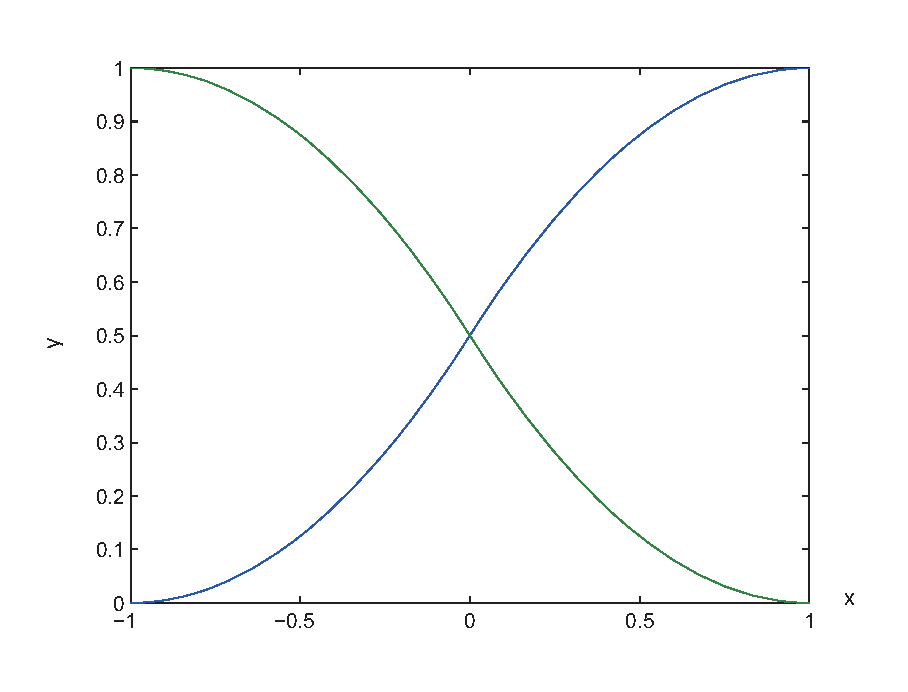
\includegraphics[width = 0.3\textwidth]{test1}
    \DeclareGraphicsExtensions.
  }
  \subfigure[$D=0.5$]{ \label{fig:ex1:resD:b}
    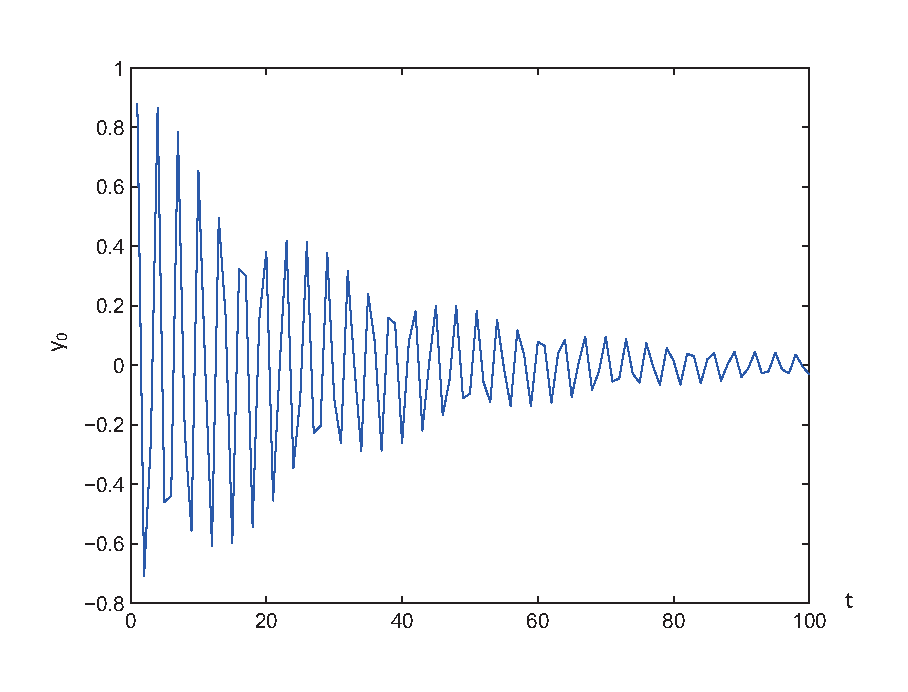
\includegraphics[width = 0.3\textwidth]{test2}
    \DeclareGraphicsExtensions.
  }
  \DeclareGraphicsExtensions.
  \caption{Test graphs.}\label{fig:ex1:resD}
\end{figure}
\end{frame}


%-------------------------------------------------------
\begin{frame}{Examples}{Equations}
%-------------------------------------------------------
\begin{itemize}
  \item Test blocked equations, i.e. \eqref{fml:eq1:partialW}, \eqref{fml:eq1:partialb}.
\end{itemize}

\begin{block}{SVM loss function}
  \label{blc:eq1} Here we show a simple example of subequations in \eqref{fml:eq1:partialW}:
  \begin{subequations}
    \renewcommand{\theequation}
    {\theparentequation-\arabic{equation}}
    \begin{align}
      \frac{\partial \mathcal{L}(\mathbf{w},~b)}{\partial \mathbf{w}} &= \mathbf{w} + C \sum\limits_i\frac{\partial \ell_i}{\partial \mathbf{w}}, \label{fml:eq1:partialW}\\
      \frac{\partial \mathcal{L}(\mathbf{w},~b)}{\partial b} &= C \sum\limits_i\frac{\partial \ell_i}{\partial b}, \label{fml:eq1:partialb}
    \end{align}
  \end{subequations}
\end{block}
\end{frame}


%-------------------------------------------------------
\begin{frame}{Examples}{Theorems}
%-------------------------------------------------------
\begin{itemize}
  \item Test theorems, i.e. \cref{thm:th1} and \cref{thm:th2}.
\end{itemize}

\begin{columns}
  \begin{column}{.48\textwidth}
    \begin{theorem}[Example Theorem 1]
      Nam dui ligula, fringilla a, euismod
      sodales, sollicitudin vel, wisi. Morbi
      auctor lorem non justo. Nam lacus
      libero, pretium at, lobortis vitae,
      ultricies et, tellus. Donec aliquet,
      tortor sed accumsan bibendum, erat
      ligula aliquet magna, vitae ornare
      odio metus a mi. \label{thm:th1}
    \end{theorem}
  \end{column}
  \begin{column}{.48\textwidth}
    \begin{theorem}[Example Theorem 2]
      Quisque ullamcorper placerat ipsum.
      Cras nibh. Morbi vel justo vitae lacus
      tincidunt ultrices. Lorem ipsum dolor
      sit amet, consectetuer adipiscing elit.
      In hac habitasse platea dictumst.
      Integer tempus convallis augue.
      Etiam facilisis. Nunc elementum
      fermentum wisi. \label{thm:th2}
    \end{theorem}
  \end{column}
\end{columns}
\end{frame}


%-------------------------------------------------------
\begin{frame}{Examples}{Algorithm}
%-------------------------------------------------------
\begin{itemize}
  \item Test algorithm, i.e. \cref{alg::Algorithm}.
\end{itemize}

\begin{algorithm}[H]
  \caption{DWT Algorithm}
  \label{alg::Algorithm}
  \begin{algorithmic}[1]
    \REQUIRE Sequence $\mathbf{x}$ in time domain
    \ENSURE Sequence $\hat{\mathbf{x}}$ in wavelet domain
    % if-then-else
    \STATE N = $\left\lfloor \log_2 (\mathrm{length}(\mathbf{x})) \right\rfloor$;
    \STATE $\mathbf{c}_{N} = \mathbf{x},~ \hat{\mathbf{x}} = \varnothing$;
    \FOR{$i$ from $1$ to $N$}
    \STATE $\mathbf{c}_{N-i},~\mathbf{d}_{N-i}~=~\mathrm{analysis\_filter}(\mathbf{c}_{N-i+1})$;
    \STATE insert $\mathbf{d}_{N-i}$ at the beginning of $\hat{\mathbf{x}}$.
    \ENDFOR
  \end{algorithmic}
\end{algorithm}
\end{frame}


\finalframe[It's time for Q\&A.]

\end{document}
